% Texto preparado para o modelo SBC usado no Overleaf.
% Substitua os campos entre colchetes antes da entrega.

\documentclass[12pt]{article}

\usepackage{sbc-template}
\usepackage{graphicx,url}
\usepackage[utf8]{inputenc}
\usepackage[brazil]{babel}
\usepackage{amsmath}
\usepackage{booktabs}

\sloppy

\title{Predição Explicável de Turnover de Funcionários com XGBoost, Validação Cruzada e SHAP}

\author{Abinoã Menezes\inst{1}, [Nome do orientador]\inst{1}}

\address{Departamento de Estatística e Informática\\
Universidade Federal Rural de Pernambuco (UFRPE)\\
Rua Dom Manuel de Medeiros, s/n -- CEP 52171-900 -- Recife -- PE -- Brasil
\email{[seu e-mail], [e-mail do orientador]}}

\begin{document}

\maketitle

\begin{resumo}
A rotatividade de funcionários pode afetar a continuidade das atividades, ampliar custos de recrutamento e treinamento e provocar perda de conhecimento organizacional. Nesse contexto, este trabalho desenvolve uma abordagem de aprendizado de máquina para estimar a probabilidade de saída de funcionários e explicar os fatores associados a cada previsão. A base analisada contém 14.999 registros, dos quais 23,81\% representam funcionários que saíram. Para reduzir vieses de avaliação, aproximadamente 20\% dos dados foram reservados como teste final, enquanto os 80\% restantes foram submetidos à validação cruzada estratificada e agrupada em cinco \textit{folds}. O agrupamento manteve registros com atributos idênticos no mesmo subconjunto, evitando que duplicatas aparecessem simultaneamente no treinamento e na avaliação. O modelo principal utiliza XGBoost, sobreamostragem aleatória aplicada exclusivamente aos dados de treinamento e \textit{early stopping}. Também foram avaliadas versões do XGBoost com peso de classe e do CatBoost. No teste final, o modelo principal alcançou 97,10\% de acurácia, 95,24\% de precisão, 92,45\% de \textit{recall}, 93,83\% de F1-score e 98,89\% de AUC-ROC para a classe de saída. A proximidade entre validação e teste não indicou sobreajuste acentuado na base estudada, embora não comprove generalização para outras organizações. Os valores SHAP foram empregados para produzir explicações globais e individuais, destacando fatores associados à satisfação, ao tempo de empresa, à quantidade de projetos e à carga horária. Uma LLM local foi integrada apenas como camada opcional de redação, sem alterar previsões ou valores SHAP. Os resultados indicam potencial de apoio à análise do setor de recursos humanos, desde que as explicações sejam interpretadas como associações do modelo e submetidas à avaliação humana.

\textbf{Palavras-chave:} turnover; aprendizado de máquina; XGBoost; validação cruzada; SHAP; inteligência artificial explicável.
\end{resumo}

\begin{abstract}
Employee turnover can disrupt business continuity, increase recruitment and training costs, and lead to the loss of organizational knowledge. This study develops a machine-learning approach to estimate employees' probability of leaving and explain the factors associated with each prediction. The analyzed dataset contains 14,999 records, of which 23.81\% represent employees who left. To reduce evaluation bias, approximately 20\% of the data were reserved as a final test set, while the remaining 80\% were evaluated through five-fold stratified group cross-validation. Grouping kept records with identical attributes within the same subset, preventing duplicates from appearing simultaneously in training and evaluation data. The main model combines XGBoost, random oversampling applied exclusively to training data, and early stopping. Class-weighted XGBoost and CatBoost alternatives were also evaluated. On the final test set, the main model achieved 97.10\% accuracy, 95.24\% precision, 92.45\% recall, a 93.83\% F1-score, and a 98.89\% ROC-AUC for the employee-leaving class. The similarity between cross-validation and test results did not indicate severe overfitting within the analyzed dataset, although it does not demonstrate generalization to other organizations. SHAP values were used to generate global and individual explanations, highlighting factors associated with satisfaction, company tenure, number of projects, and workload. A local large language model was integrated only as an optional text-generation layer, without changing predictions or SHAP values. The results demonstrate the approach's potential to support human-resources analysis, provided that explanations are treated as model associations and remain subject to human review.

\textbf{Keywords:} employee turnover; machine learning; XGBoost; cross-validation; SHAP; explainable artificial intelligence.
\end{abstract}

\section{Introdução}

\subsection{Contexto}

A rotatividade de funcionários, também denominada \textit{turnover}, faz parte da dinâmica das organizações e ocorre quando profissionais deixam a empresa por iniciativa própria ou por decisão institucional. Quando esse processo acontece de maneira frequente ou inesperada, pode comprometer a continuidade das atividades, provocar perda de conhecimento interno e gerar novas demandas de recrutamento, seleção e treinamento. A literatura sobre o tema evoluiu de tentativas de controle da rotatividade para modelos que investigam atitudes, permanência, trajetórias e efeitos coletivos da saída de profissionais \cite{hom2017turnover}.

A crescente disponibilidade de dados organizacionais permite que o setor de recursos humanos complemente suas análises com técnicas computacionais. Informações sobre satisfação, carga de trabalho, tempo de empresa, projetos, avaliações e progressão profissional podem conter padrões associados à permanência ou à saída. Uma revisão sistemática de 52 estudos publicados entre 2012 e abril de 2023 identificou mais de vinte técnicas de aprendizado de máquina aplicadas à predição de \textit{turnover}, com predomínio de abordagens supervisionadas \cite{akasheh2024decade}. Esses resultados mostram a relevância do tema, mas também revelam diversidade de dados, protocolos experimentais e métricas, o que exige cautela ao comparar desempenhos.

\subsection{Problema e motivação}

Este trabalho trata o \textit{turnover} como um problema de classificação binária. Para cada registro de funcionário, representado por um vetor de características $\mathbf{x}$, busca-se aprender uma função $f(\mathbf{x})$ que estime a probabilidade de a classe ser SAIU ($y=1$), em oposição a FICOU ($y=0$):

\begin{equation}
f(\mathbf{x}) \approx P(Y=1\mid \mathbf{X}=\mathbf{x}).
\end{equation}

A aplicação apresenta desafios metodológicos. Primeiro, a classe SAIU é minoritária, correspondendo a 23,81\% da base. Um classificador pode alcançar acurácia aparentemente elevada ao favorecer a classe FICOU, sem identificar adequadamente as saídas. Segundo, a presença de registros repetidos pode inflar a avaliação caso cópias de uma mesma combinação de atributos sejam distribuídas entre treinamento e teste. Terceiro, algoritmos de alto desempenho, como os baseados em conjuntos de árvores, não produzem explicações imediatamente compreensíveis para profissionais de RH.

Por esses motivos, o problema não se resume a maximizar acurácia. É necessário medir especificamente o desempenho sobre a classe SAIU, prevenir vazamento de dados, avaliar a estabilidade em divisões diferentes e explicar os fatores que contribuíram para cada resultado. Também é necessário preservar o papel humano: uma probabilidade ou uma explicação do modelo não comprova a causa de uma saída e não deve fundamentar, isoladamente, demissão, promoção, remuneração ou qualquer decisão com efeito sobre o trabalhador.

\subsection{Objetivos}

O objetivo geral é desenvolver e avaliar uma abordagem explicável de aprendizado de máquina para estimar o risco de \textit{turnover} e apoiar a investigação do setor de recursos humanos.

Os objetivos específicos são:

\begin{itemize}
    \item caracterizar e preparar a base de dados utilizada;
    \item tratar o desbalanceamento sem modificar os conjuntos de validação e teste;
    \item impedir que registros com atributos idênticos sejam separados entre treinamento e avaliação;
    \item avaliar a generalização com validação cruzada e um teste final reservado;
    \item comparar sobreamostragem aleatória e ponderação de classe, bem como XGBoost e CatBoost;
    \item investigar sinais de sobreajuste por meio das diferenças entre treinamento, validação e teste;
    \item produzir explicações SHAP globais e individuais; e
    \item apresentar os resultados como apoio à decisão, mantendo revisão humana e explicitando limitações.
\end{itemize}

\subsection{Visão geral da abordagem}

A abordagem principal utiliza XGBoost com codificação das variáveis categóricas, sobreamostragem da classe SAIU apenas no treinamento e seleção da quantidade de árvores por \textit{early stopping}. Aproximadamente 20\% da base permanecem intocados até o teste final. Os 80\% restantes são usados em uma validação cruzada estratificada e agrupada com cinco \textit{folds}. A estratificação procura preservar a proporção das classes; o agrupamento mantém atributos idênticos na mesma partição.

Além do modelo principal, são avaliados XGBoost com peso na classe SAIU, sem duplicação de registros, e CatBoost com peso de classe e processamento nativo das características categóricas. Após a avaliação, contribuições SHAP são calculadas para o modelo XGBoost. Uma visão global resume padrões do conjunto, enquanto uma visão local mostra por que um caso específico recebeu determinada previsão. Uma LLM executada localmente pode selecionar uma orientação curta entre ações previamente permitidas para o RH, mas os números e fatores permanecem produzidos deterministicamente pelo programa.

\subsection{Contribuições}

As principais contribuições do trabalho são: (i) um protocolo de avaliação que separa teste final e validação cruzada; (ii) o agrupamento conservador de registros idênticos para reduzir contaminação; (iii) a comparação entre estratégias de tratamento do desbalanceamento; (iv) a avaliação conjunta de acurácia, precisão, \textit{recall}, F1, AUC-ROC e matriz de confusão; e (v) a integração de predição e explicabilidade em uma estrutura de apoio ao RH.

Do ponto de vista prático, a apresentação foi organizada em camadas. O RH pode começar pelo gráfico global, avançar para a comparação entre departamentos e faixas salariais e consultar explicações individuais somente quando necessário. O comparativo apresenta fatores em comum uma única vez por dimensão e destaca as diferenças em uma tabela curta, reduzindo a repetição de textos extensos.

\subsection{Organização do trabalho}

O restante do texto está organizado da seguinte forma. A Seção~\ref{sec:referencial} apresenta os fundamentos. A Seção~\ref{sec:relacionados} discute trabalhos relacionados. A Seção~\ref{sec:abordagem} descreve a abordagem. A Seção~\ref{sec:experimentos} detalha os experimentos. A Seção~\ref{sec:resultados} apresenta os resultados e sua interpretação. Por fim, a Seção~\ref{sec:conclusoes} reúne conclusões, limitações e trabalhos futuros.

\section{Referencial teórico}
\label{sec:referencial}

\subsection{Turnover e análise de pessoas}

O termo \textit{turnover} abrange movimentos de saída de trabalhadores em relação a uma organização. A saída pode ser voluntária ou involuntária, e sua interpretação depende do contexto. A pesquisa organizacional acumulou diferentes teorias para explicar por que pessoas deixam ou permanecem, incluindo satisfação, comprometimento, alternativas externas e inserção no trabalho \cite{hom2017turnover}. Um modelo preditivo não substitui essas teorias: ele identifica regularidades estatísticas nos atributos disponíveis.

Na análise de pessoas, dados administrativos podem permitir estimativas sem exigir pesquisas adicionais. Rombaut e Guerry demonstraram, em dados reais de uma empresa, que registros de sistemas de RH podem apoiar previsões de rotatividade e a identificação de grupos de risco \cite{rombaut2018predicting}. No entanto, o valor operacional depende da qualidade dos dados e da correspondência entre as variáveis registradas e o fenômeno que se deseja analisar.

\subsection{Aprendizado supervisionado e classificação}

No aprendizado supervisionado, o algoritmo recebe exemplos com atributos e classes conhecidas para aprender uma regra de predição. Neste trabalho, $y=1$ representa SAIU e $y=0$ representa FICOU. A probabilidade estimada é convertida em classe por um limiar $\tau=0{,}5$:

\begin{equation}
\widehat{y}=\begin{cases}
1, & \text{se } f(\mathbf{x})\geq \tau,\\
0, & \text{caso contrário.}
\end{cases}
\end{equation}

O limiar de 0,5 é uma referência inicial, e não necessariamente o melhor valor para operação. Em uma implantação real, sua escolha deve considerar o custo de não identificar uma saída e o custo de encaminhar ao RH uma pessoa que permaneceria.

\subsection{XGBoost e CatBoost}

O XGBoost é uma implementação escalável de \textit{gradient tree boosting}. Em vez de construir uma única árvore, o método adiciona árvores sequencialmente para corrigir erros do conjunto anterior. De forma simplificada, na iteração $t$ a predição é dada por

\begin{equation}
\widehat{y}^{(t)}_i=\widehat{y}^{(t-1)}_i+f_t(\mathbf{x}_i),
\end{equation}

e a função objetivo combina perda preditiva e regularização da complexidade:

\begin{equation}
\mathcal{L}^{(t)}=\sum_{i=1}^{n}l\left(y_i,\widehat{y}^{(t-1)}_i+f_t(\mathbf{x}_i)\right)+\Omega(f_t).
\end{equation}

A regularização, a taxa de aprendizado e o controle de profundidade ajudam a limitar a complexidade. O XGBoost também foi projetado com otimizações para esparsidade e eficiência computacional \cite{chen2016xgboost}.

O CatBoost é outro método de \textit{gradient boosting}, criado com técnicas específicas para variáveis categóricas e \textit{ordered boosting}. Seu processamento busca reduzir formas de vazamento e deslocamento de predição relacionadas ao uso de estatísticas do alvo em categorias \cite{prokhorenkova2018catboost}. Neste trabalho, ele atua como comparação porque Departamento e Faixa Salarial são categóricas.

\subsection{Desbalanceamento das classes}

Uma base é desbalanceada quando as classes têm quantidades diferentes de exemplos. A proporção de 76,19\% FICOU e 23,81\% SAIU não impede o treinamento, mas pode influenciar a fronteira de decisão. A primeira estratégia avaliada foi o \textit{RandomOverSampler}, que seleciona exemplos da minoria aleatoriamente, com reposição, até igualar as classes \cite{lemaitre2017imbalanced}. Para evitar vazamento, a sobreamostragem deve ser executada depois da divisão e somente no treino de cada \textit{fold}.

A segunda estratégia foi atribuir maior peso aos erros da classe SAIU. No XGBoost, o parâmetro \texttt{scale\_pos\_weight} recebeu a razão entre as quantidades de FICOU e SAIU no treinamento, aproximadamente 3,2. Essa alternativa não cria cópias. A comparação empírica é importante porque nenhuma estratégia é universalmente superior.

\subsection{Validação cruzada e prevenção de vazamento}

Na validação cruzada $k$-\textit{fold}, o conjunto de desenvolvimento é dividido em $k$ partes. Em cada rodada, uma parte é usada para validação e as demais para treinamento. A repetição permite observar média e variabilidade, em vez de depender de uma única divisão \cite{kohavi1995crossvalidation}. A estratificação procura conservar a distribuição das classes.

Neste estudo, a validação também é agrupada. Cada combinação de atributos recebe um identificador de grupo, e grupos não podem ser divididos entre treino e validação. O procedimento é conservador: como a base não possui ID de funcionário, não é possível saber se duas linhas idênticas representam repetição do mesmo indivíduo ou pessoas diferentes. Ainda assim, mantê-las juntas reduz o risco de o modelo ser avaliado sobre uma cópia de algo visto no treinamento.

\subsection{Métricas de avaliação}

Considerando SAIU como classe positiva, verdadeiro positivo (VP) é uma saída corretamente prevista; falso negativo (FN) é uma saída prevista como permanência; falso positivo (FP) é uma permanência prevista como saída; e verdadeiro negativo (VN) é uma permanência corretamente prevista. As métricas usadas são:

\begin{align}
\text{Acurácia} &= \frac{VP+VN}{VP+VN+FP+FN},\\
\text{Precisão} &= \frac{VP}{VP+FP},\\
\text{Recall} &= \frac{VP}{VP+FN},\\
F1 &= 2\frac{\text{Precisão}\cdot\text{Recall}}{\text{Precisão}+\text{Recall}},\\
\text{Especificidade} &= \frac{VN}{VN+FP}.
\end{align}

A AUC-ROC resume a capacidade de ordenar positivos acima de negativos ao variar o limiar. Para uma classe minoritária relevante, acurácia isolada não é suficiente. O \textit{recall} indica quantas saídas reais foram identificadas, enquanto a precisão informa quantas previsões de saída estavam corretas.

\subsection{Explicabilidade com SHAP}

SHAP é uma família de métodos de atribuição baseada em valores de Shapley. Cada característica recebe uma contribuição $\phi_j$ para afastar a saída do modelo de um valor-base $\phi_0$ \cite{lundberg2017shap}:

\begin{equation}
f(\mathbf{x})=\phi_0+\sum_{j=1}^{M}\phi_j.
\end{equation}

Para conjuntos de árvores, o TreeSHAP permite calcular atribuições consistentes e localmente exatas de forma eficiente \cite{lundberg2020treeshap}. A implementação deste trabalho usa as contribuições nativas do XGBoost por meio de \texttt{pred\_contribs=True}. Na classificação binária, elas são expressas na margem não transformada, em \textit{log-odds}. Valores positivos elevam a margem da classe SAIU; valores negativos a reduzem. Isso não significa que a unidade original da variável seja \textit{log-odds} nem que a característica seja causa da saída.

Uma explicação local descreve um registro. Uma explicação global pode ser obtida agregando magnitudes ou exibindo a distribuição das contribuições de vários registros. Pesquisas recentes defendem uma análise em camadas, incluindo importância global, efeitos, interações, explicações locais e coortes, além de calibração e auditoria de equidade \cite{jia2026explainable}. Essa visão orienta a evolução proposta para o protótipo.

\section{Trabalhos relacionados}
\label{sec:relacionados}

Sexton et al. aplicaram redes neurais combinadas a um algoritmo genético modificado para prever saídas voluntárias e identificar entradas relevantes \cite{sexton2005turnover}. O estudo é representativo de uma fase em que a prioridade era demonstrar que o fenômeno poderia ser previsto por modelos não lineares. Embora a proposta buscasse parcimônia, explicações por atribuição local ainda não eram o foco.

Rombaut e Guerry utilizaram regressão logística e árvore de decisão sobre registros reais de RH de uma empresa belga \cite{rombaut2018predicting}. A regressão forneceu probabilidades individuais, enquanto a árvore ajudou a identificar grupos de risco. Essa combinação é particularmente relevante para este trabalho porque mostra que o consumo da informação pelo RH pode ocorrer tanto no nível individual quanto no coletivo.

Al Akasheh et al. revisaram 52 estudos sobre predição de rotatividade publicados ao longo de uma década \cite{akasheh2024decade}. Os autores encontraram predominância de aprendizado supervisionado e destacaram salário e horas extras entre fatores recorrentes. A revisão também evidencia que diferenças entre bases e protocolos dificultam transformar o melhor resultado de um estudo em uma escolha universal de algoritmo.

Nassreddine et al. avaliaram modelos de conjunto, sobreamostragem aleatória, seleção de atributos por SHAP e explicações locais em duas bases públicas, incluindo a base Kaggle com 14.999 registros \cite{nassreddine2026attrition}. Os autores observaram que métodos mais complexos de reamostragem não produziram ganhos estatisticamente significativos sobre a sobreamostragem aleatória no contexto estudado. Esse trabalho é próximo à presente pesquisa pela combinação entre desbalanceamento, modelos de árvores e explicabilidade.

Qin et al. propuseram um conjunto ponderado de LightGBM e XGBoost combinado a SHAP, obtendo AUC de 0,9504 em seu cenário experimental \cite{qin2026turnover}. O trabalho enfatiza a passagem de uma previsão opaca para informação interpretável ao RH. Entretanto, os próprios resultados da literatura não devem ser comparados diretamente aos deste estudo sem considerar diferenças de base, partição e classe positiva.

Jia propôs um protocolo explicável em quatro camadas, combinando importância global, efeito das características, interações, explicações locais e análise por coortes \cite{jia2026explainable}. O estudo também inclui calibração de limiar, auditoria de equidade e validação externa. O presente protótipo inclui uma comparação descritiva entre departamentos e faixas salariais, mas ainda precisa avaliar sua utilidade com profissionais de RH e testar a abordagem em dados externos.

Em relação a esses trabalhos, esta pesquisa concentra sua contribuição na disciplina experimental aplicada a uma base com duplicatas, na comparação de formas de tratar o desbalanceamento e na integração entre resultado preditivo e explicações destinadas ao uso humano. Não se afirma que o modelo descobriu causas universais de \textit{turnover}; busca-se construir uma prova de conceito reproduzível e explicitar as condições necessárias para seu uso responsável.

\section{Abordagem proposta}
\label{sec:abordagem}

\subsection{Fluxo geral}

O fluxo possui sete etapas: leitura e inspeção da base; definição de grupos de duplicatas; separação do teste final; validação cruzada no conjunto de desenvolvimento; treinamento final; avaliação; e geração de explicações. A semente 42 é usada para tornar as divisões reproduzíveis.

A separação externa usa cinco partes estratificadas e agrupadas, das quais a primeira é reservada como teste. Isso produz 11.999 registros de desenvolvimento e 3.000 de teste. Nenhuma métrica do teste é usada para escolher a quantidade de árvores. No conjunto de desenvolvimento, cinco rodadas internas alternam validação e treinamento.

\subsection{Pré-processamento}

As variáveis Departamento e Faixa Salarial são codificadas por \textit{one-hot encoding}, removendo a primeira categoria para evitar uma coluna redundante. O codificador é ajustado exclusivamente no treino de cada rodada e depois aplicado à validação. Variáveis numéricas são mantidas em sua escala original, pois árvores de decisão não dependem de padronização para definir cortes.

No modelo principal, a classe minoritária é duplicada somente depois desse particionamento. Cada treino interno passa de aproximadamente 9.600 para 14.628 ou 14.630 exemplos balanceados, com 50\% de cada classe. A validação permanece com aproximadamente 23,8\% de saídas, assim como o teste final.

\subsection{Treinamento e seleção do número de árvores}

O XGBoost principal utiliza profundidade máxima 5, taxa de aprendizado 0,1, até 1.000 árvores, função de perda logística e paralelismo disponível. O \textit{early stopping} interrompe o treinamento após 30 rodadas sem melhora na perda de validação. Os cinco números selecionados foram 151, 214, 191, 85 e 161 árvores. A mediana, 161, foi usada no treinamento final por ser menos sensível a uma rodada que pare muito cedo ou tarde.

No experimento ponderado, o XGBoost recebe peso positivo calculado apenas no treino. No CatBoost, são usados profundidade 5, taxa 0,1, até 1.000 iterações, peso de classe e processamento categórico nativo. Todos os experimentos usam as mesmas divisões externas e internas, permitindo comparação sob condições semelhantes.

\subsection{Explicação e apoio ao RH}

As contribuições SHAP são calculadas no teste final. Para cada registro com probabilidade de saída maior ou igual a 50\%, o relatório apresenta os três maiores valores SHAP positivos e associa cada variável a um ponto de investigação previamente definido. Casos abaixo do limiar recebem apenas acompanhamento regular, evitando recomendar uma ação individual para toda a base.

O componente de linguagem usa o modelo local Llama 3.2 de 3 bilhões de parâmetros, executado pelo Ollama. Para reduzir risco de alteração de números e afirmações não sustentadas, a probabilidade, os fatores e os valores SHAP são inseridos por um texto determinístico. A LLM seleciona uma orientação curta que deve corresponder literalmente a uma ação permitida; respostas fora dessa lista são rejeitadas. Ela não tem acesso a nome, ID, classe real ou linha do funcionário, não participa da previsão e possui texto determinístico de contingência caso esteja indisponível.

Para uso prático, propõe-se organizar a interface em três níveis. O primeiro mostra o gráfico global. O segundo deve agrupar pessoas com combinações semelhantes de fatores, exibindo as características comuns uma única vez, quantidade de pessoas, risco médio e diferenças relevantes. O terceiro permite detalhar um caso. O segundo nível ainda é trabalho em andamento; portanto, os resultados atuais não devem ser descritos como um painel operacional completo.

\section{Experimentos}
\label{sec:experimentos}

\subsection{Conjunto de dados}

Foi utilizado o arquivo público \texttt{HR\_comma\_sep.csv}, associado à base HR Analytics divulgada no Kaggle \cite{kaggleHR}. Ele contém 14.999 registros, nove atributos preditores e o alvo \texttt{left}. Não há valores ausentes. A Tabela~\ref{tab:variaveis} resume os campos.

\begin{table}[ht]
\centering
\caption{Variáveis da base de dados.}
\label{tab:variaveis}
\small
\begin{tabular}{ll}
\toprule
Variável & Descrição \\
\midrule
\texttt{satisfaction\_level} & nível de satisfação, entre 0 e 1 \\
\texttt{last\_evaluation} & resultado da última avaliação \\
\texttt{number\_project} & quantidade de projetos \\
\texttt{average\_montly\_hours} & média mensal de horas \\
\texttt{time\_spend\_company} & tempo de empresa \\
\texttt{Work\_accident} & indicador de acidente de trabalho \\
\texttt{promotion\_last\_5years} & promoção nos últimos cinco anos \\
\texttt{Department} & departamento \\
\texttt{salary} & faixa salarial \\
\texttt{left} & alvo: 0=FICOU; 1=SAIU \\
\bottomrule
\end{tabular}
\end{table}

Há 11.428 registros FICOU (76,19\%) e 3.571 SAIU (23,81\%). Foram encontradas 3.008 ocorrências repetidas além da primeira ocorrência de cada combinação idêntica. A base não contém ID, data de observação, data de saída, organização de origem ou descrição do instrumento de coleta. Assim, não é possível acompanhar uma pessoa no tempo, distinguir com certeza duplicação de indivíduos de coincidência de atributos ou realizar divisão temporal.

\subsection{Protocolo de avaliação}

O teste final preserva 3.000 registros: 2.285 FICOU e 715 SAIU. Os 11.999 registros restantes formam o desenvolvimento. Cada validação interna contém cerca de 2.400 registros com 23,8\% de saídas. O desempenho é calculado para treino e validação em cada rodada; o teste é consultado apenas após a definição do número final de árvores.

A implementação foi realizada em Python, com Scikit-learn para pré-processamento, partições e métricas \cite{pedregosa2011scikit}, Imbalanced-learn para sobreamostragem, além das bibliotecas XGBoost, CatBoost, Pandas, NumPy e Matplotlib. Os experimentos foram executados com semente fixa para permitir reprodução das divisões.

São comparados três cenários:

\begin{enumerate}
    \item XGBoost com sobreamostragem aleatória no treinamento;
    \item XGBoost sem sobreamostragem e com peso na classe SAIU; e
    \item CatBoost com peso na classe SAIU.
\end{enumerate}

A classe positiva é sempre SAIU. O limiar é 0,5. Não foi realizada busca extensiva de hiperparâmetros, o que reduz risco de ajuste excessivo ao protocolo, mas significa que os resultados não representam necessariamente o melhor desempenho alcançável.

\section{Resultados e discussão}
\label{sec:resultados}

\subsection{Validação cruzada do modelo principal}

A Tabela~\ref{tab:folds} mostra o resultado do XGBoost com sobreamostragem. As métricas são percentuais. A acurácia variou de 96,96\% a 97,62\%, e o \textit{recall} da classe SAIU variou de 90,37\% a 94,06\%.

\begin{table}[ht]
\centering
\caption{Resultados da validação cruzada do modelo principal.}
\label{tab:folds}
\small
\begin{tabular}{cccccc}
\toprule
Fold & Acurácia & Precisão & Recall & F1 & AUC \\
\midrule
1 & 97,29 & 95,18 & 93,35 & 94,25 & 98,35 \\
2 & 97,62 & 95,89 & 94,05 & 94,96 & 98,95 \\
3 & 97,29 & 94,55 & 94,06 & 94,30 & 98,92 \\
4 & 96,96 & 96,63 & 90,37 & 93,39 & 97,73 \\
5 & 97,58 & 96,72 & 92,99 & 94,82 & 98,72 \\
\midrule
Média & 97,35 & 95,79 & 92,96 & 94,35 & 98,53 \\
Desvio & 0,24 & 0,84 & 1,36 & 0,55 & 0,46 \\
\bottomrule
\end{tabular}
\end{table}

O quarto \textit{fold} apresentou o menor \textit{recall} e a maior precisão da classe SAIU. Isso não é contraditório. Houve apenas 18 falsos positivos, o que elevou a precisão, mas 55 falsos negativos, o que reduziu o \textit{recall}. O exemplo reforça por que uma única métrica não descreve todo o comportamento do modelo.

No treinamento, as médias foram 98,89\% de acurácia, 97,95\% de precisão, 97,38\% de \textit{recall}, 97,66\% de F1 e 99,87\% de AUC. A diferença de acurácia entre treino e validação foi de 1,54 ponto percentual, enquanto a diferença de \textit{recall} foi de 4,42 pontos. Existe uma queda esperada fora do treino, mais visível no \textit{recall}, mas não um colapso de desempenho.

\subsection{Teste final}

No teste reservado, a matriz de confusão do modelo principal foi:

\begin{table}[ht]
\centering
\caption{Matriz de confusão do teste final.}
\label{tab:matrizteste}
\begin{tabular}{lcc}
\toprule
Situação real & Previu SAIU & Previu FICOU \\
\midrule
SAIU & 661 (VP) & 54 (FN) \\
FICOU & 33 (FP) & 2.252 (VN) \\
\bottomrule
\end{tabular}
\end{table}

O modelo identificou 92,45\% das 715 saídas e classificou incorretamente como saída 1,44\% das 2.285 permanências. A acurácia de 97,10\% ficou próxima da média de 97,35\% da validação. A AUC-ROC de 98,89\% também ficou próxima da média de 98,53\%. Esses resultados não indicam sobreajuste acentuado dentro desta base. Contudo, a conclusão correta é limitada: estabilidade interna não equivale a validação externa.

\subsection{Comparação de algoritmos e tratamento do desbalanceamento}

A Tabela~\ref{tab:comparacao} compara os testes finais. As divisões são as mesmas nos três cenários.

\begin{table}[ht]
\centering
\caption{Comparação no teste final (\%).}
\label{tab:comparacao}
\small
\begin{tabular}{lccccc}
\toprule
Modelo & Acurácia & Precisão & Recall & F1 & AUC \\
\midrule
XGBoost + sobreamostragem & 97,100 & 95,240 & 92,450 & 93,830 & 98,890 \\
XGBoost + peso de classe & 97,567 & 97,067 & 92,587 & 94,775 & 98,677 \\
CatBoost + peso de classe & 96,533 & 92,608 & 92,867 & 92,737 & 98,751 \\
\bottomrule
\end{tabular}
\end{table}

O XGBoost ponderado obteve a maior acurácia, precisão e F1, com 662 VP, 53 FN, 20 FP e 2.265 VN. Em comparação ao principal, reduziu falsos positivos de 33 para 20 e falsos negativos de 54 para 53. O CatBoost alcançou o maior \textit{recall}, 92,87\%, identificando 664 saídas, mas gerou 53 falsos positivos e menor precisão. O modelo principal apresentou a maior AUC.

As diferenças são pequenas e ainda não foram submetidas a um teste estatístico pareado ou a validação repetida. Portanto, não se deve concluir que um algoritmo é universalmente superior. Se o objetivo priorizar equilíbrio entre precisão e \textit{recall}, o XGBoost ponderado é o candidato mais forte nesta execução. Se o custo de um falso negativo for muito maior, o CatBoost merece avaliação de limiar. A migração da camada SHAP para o XGBoost ponderado e uma comparação repetida constituem passos seguintes.

\subsection{Explicações SHAP}

A Figura~\ref{fig:shapglobal} apresenta a distribuição global das contribuições. No eixo horizontal, valores positivos elevam a margem da classe SAIU e valores negativos a reduzem. As cores representam valores relativos baixos e altos da característica. Satisfação, tempo de empresa, quantidade de projetos, média mensal de horas e última avaliação aparecem entre os atributos de maior influência global.

\begin{figure}[ht]
\centering
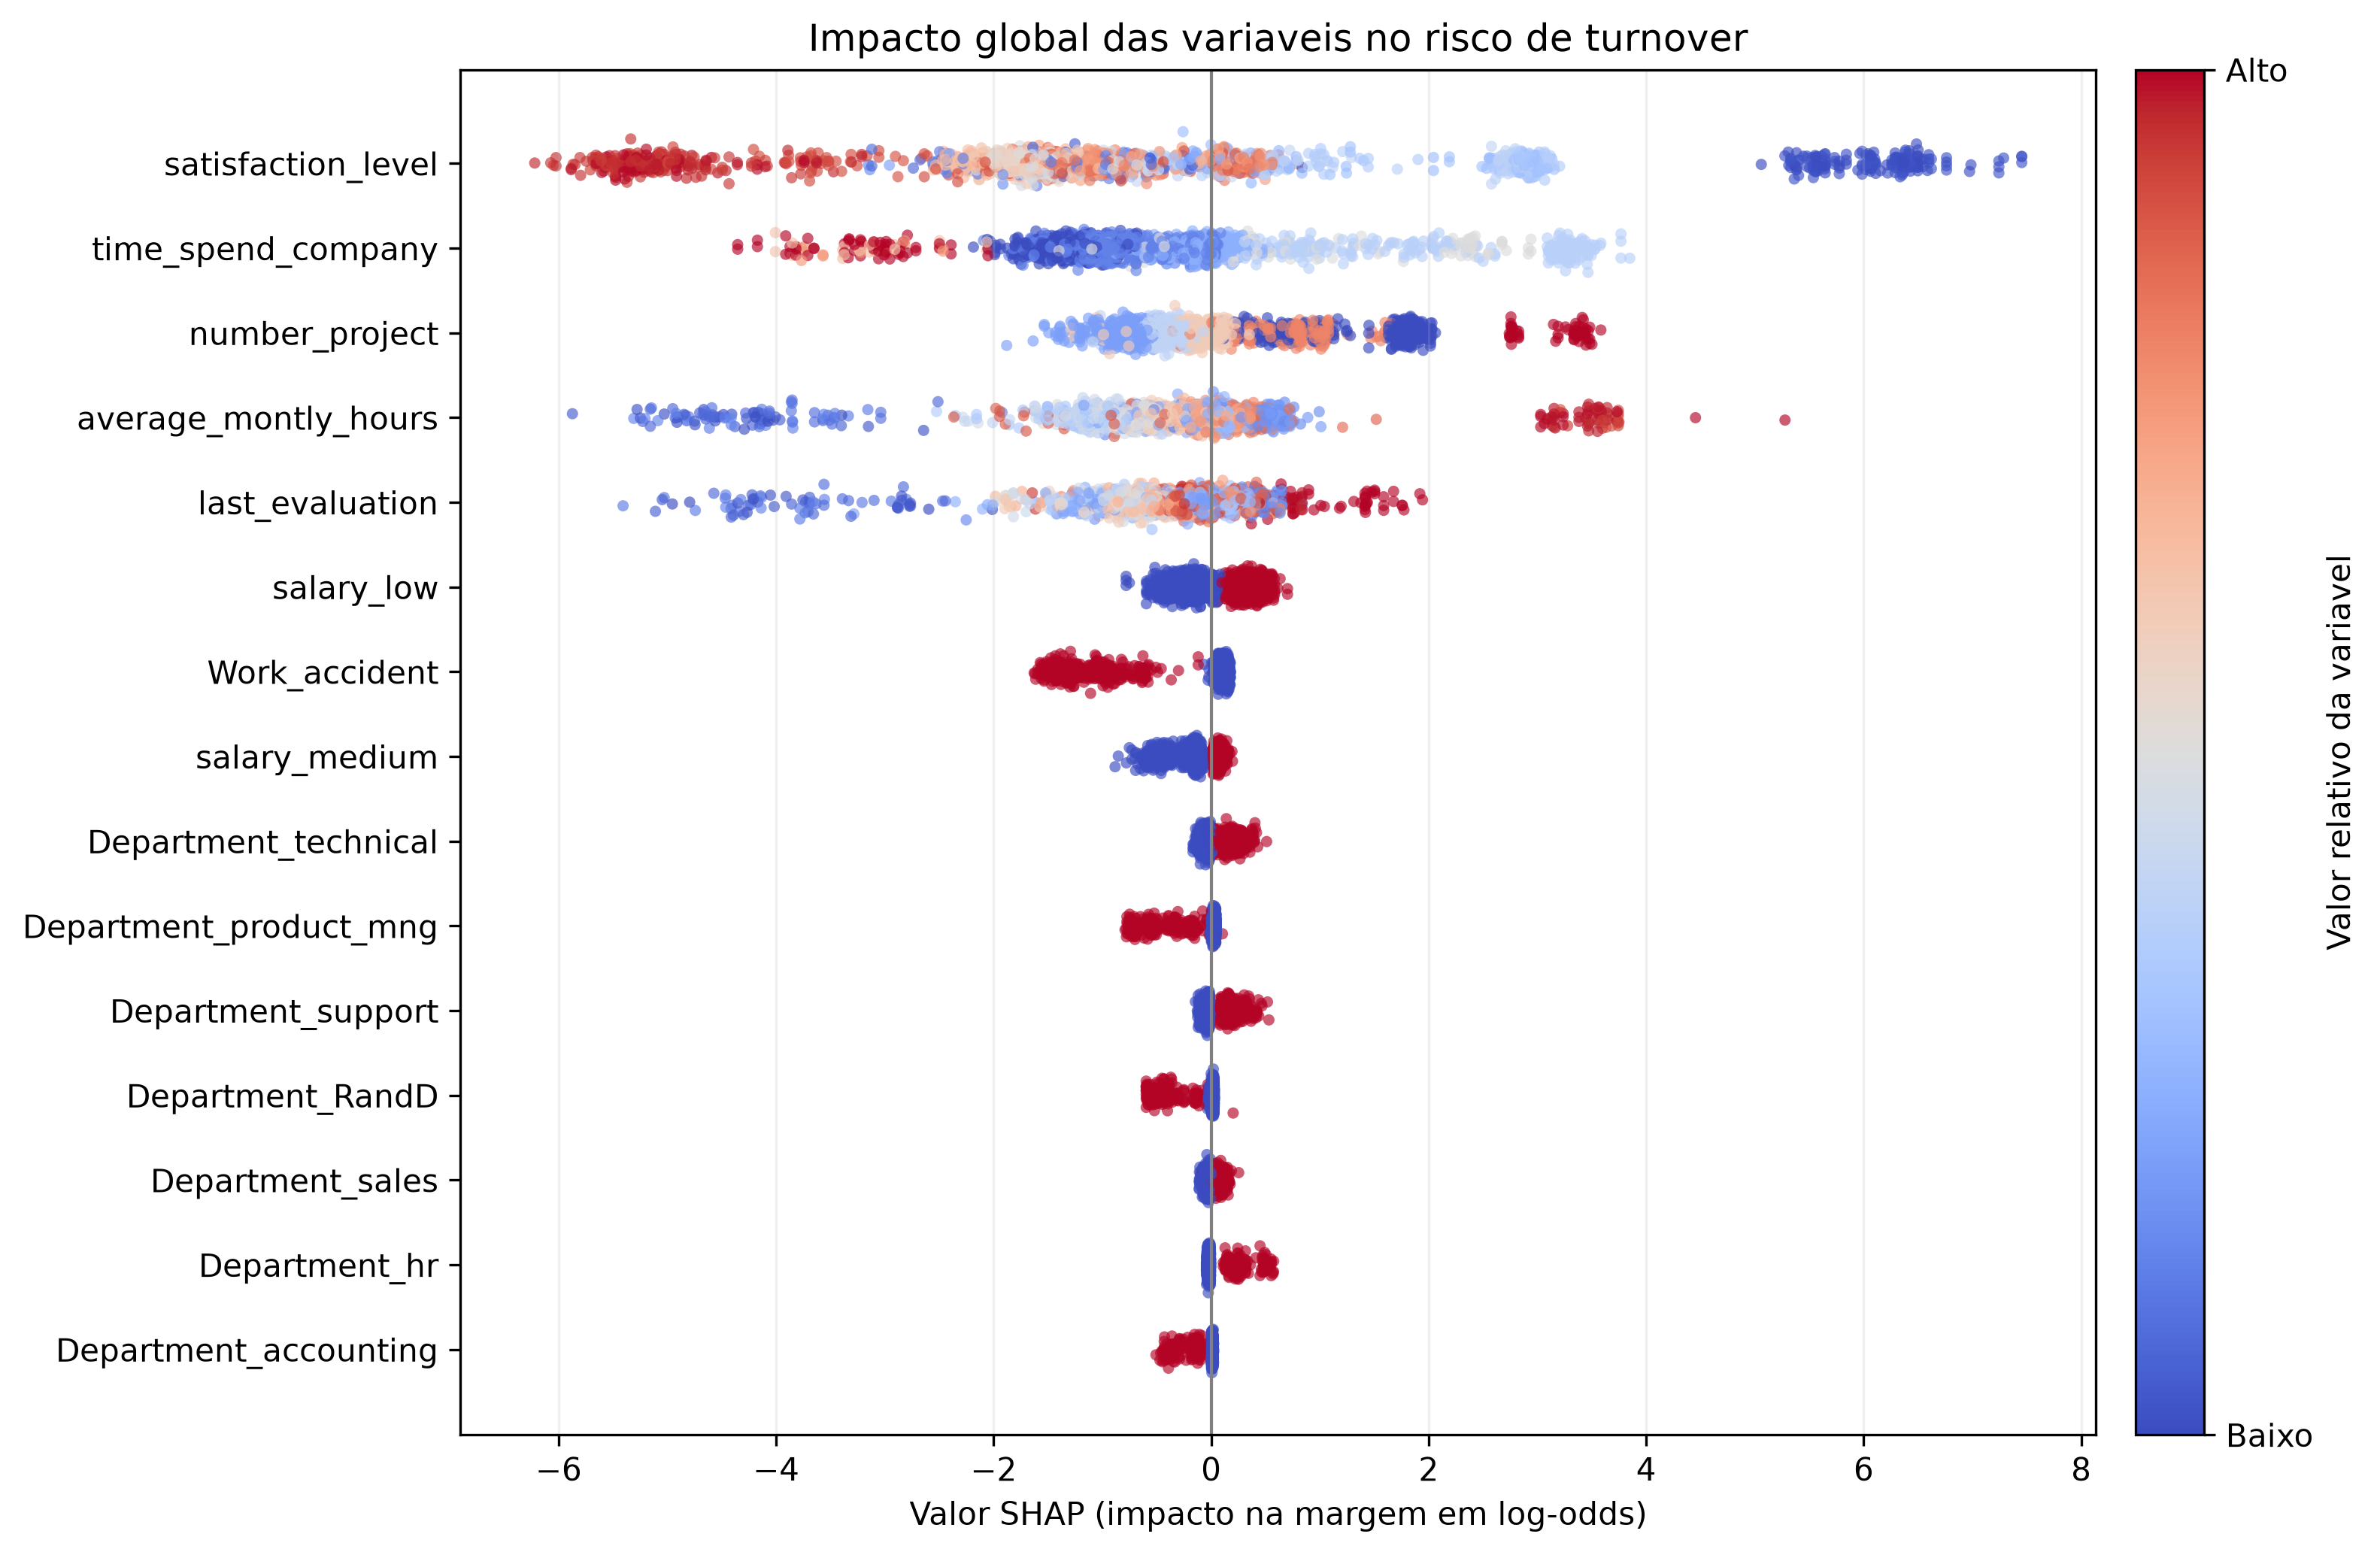
\includegraphics[width=\textwidth]{resultados/shap_summary_xgboost_kfold.png}
\caption{Impacto global das variáveis segundo valores SHAP.}
\label{fig:shapglobal}
\end{figure}

No caso individual de maior risco ilustrado na Figura~\ref{fig:shaplocal}, satisfação igual a 0,09, média mensal de 309 horas e sete projetos apresentaram contribuições positivas de aproximadamente 5,382, 3,030 e 2,756 \textit{log-odds}. A última avaliação apresentou contribuição negativa de $-0,328$. A probabilidade exibida como 100,00\% é um arredondamento e não deve ser interpretada como certeza absoluta.

\begin{figure}[ht]
\centering
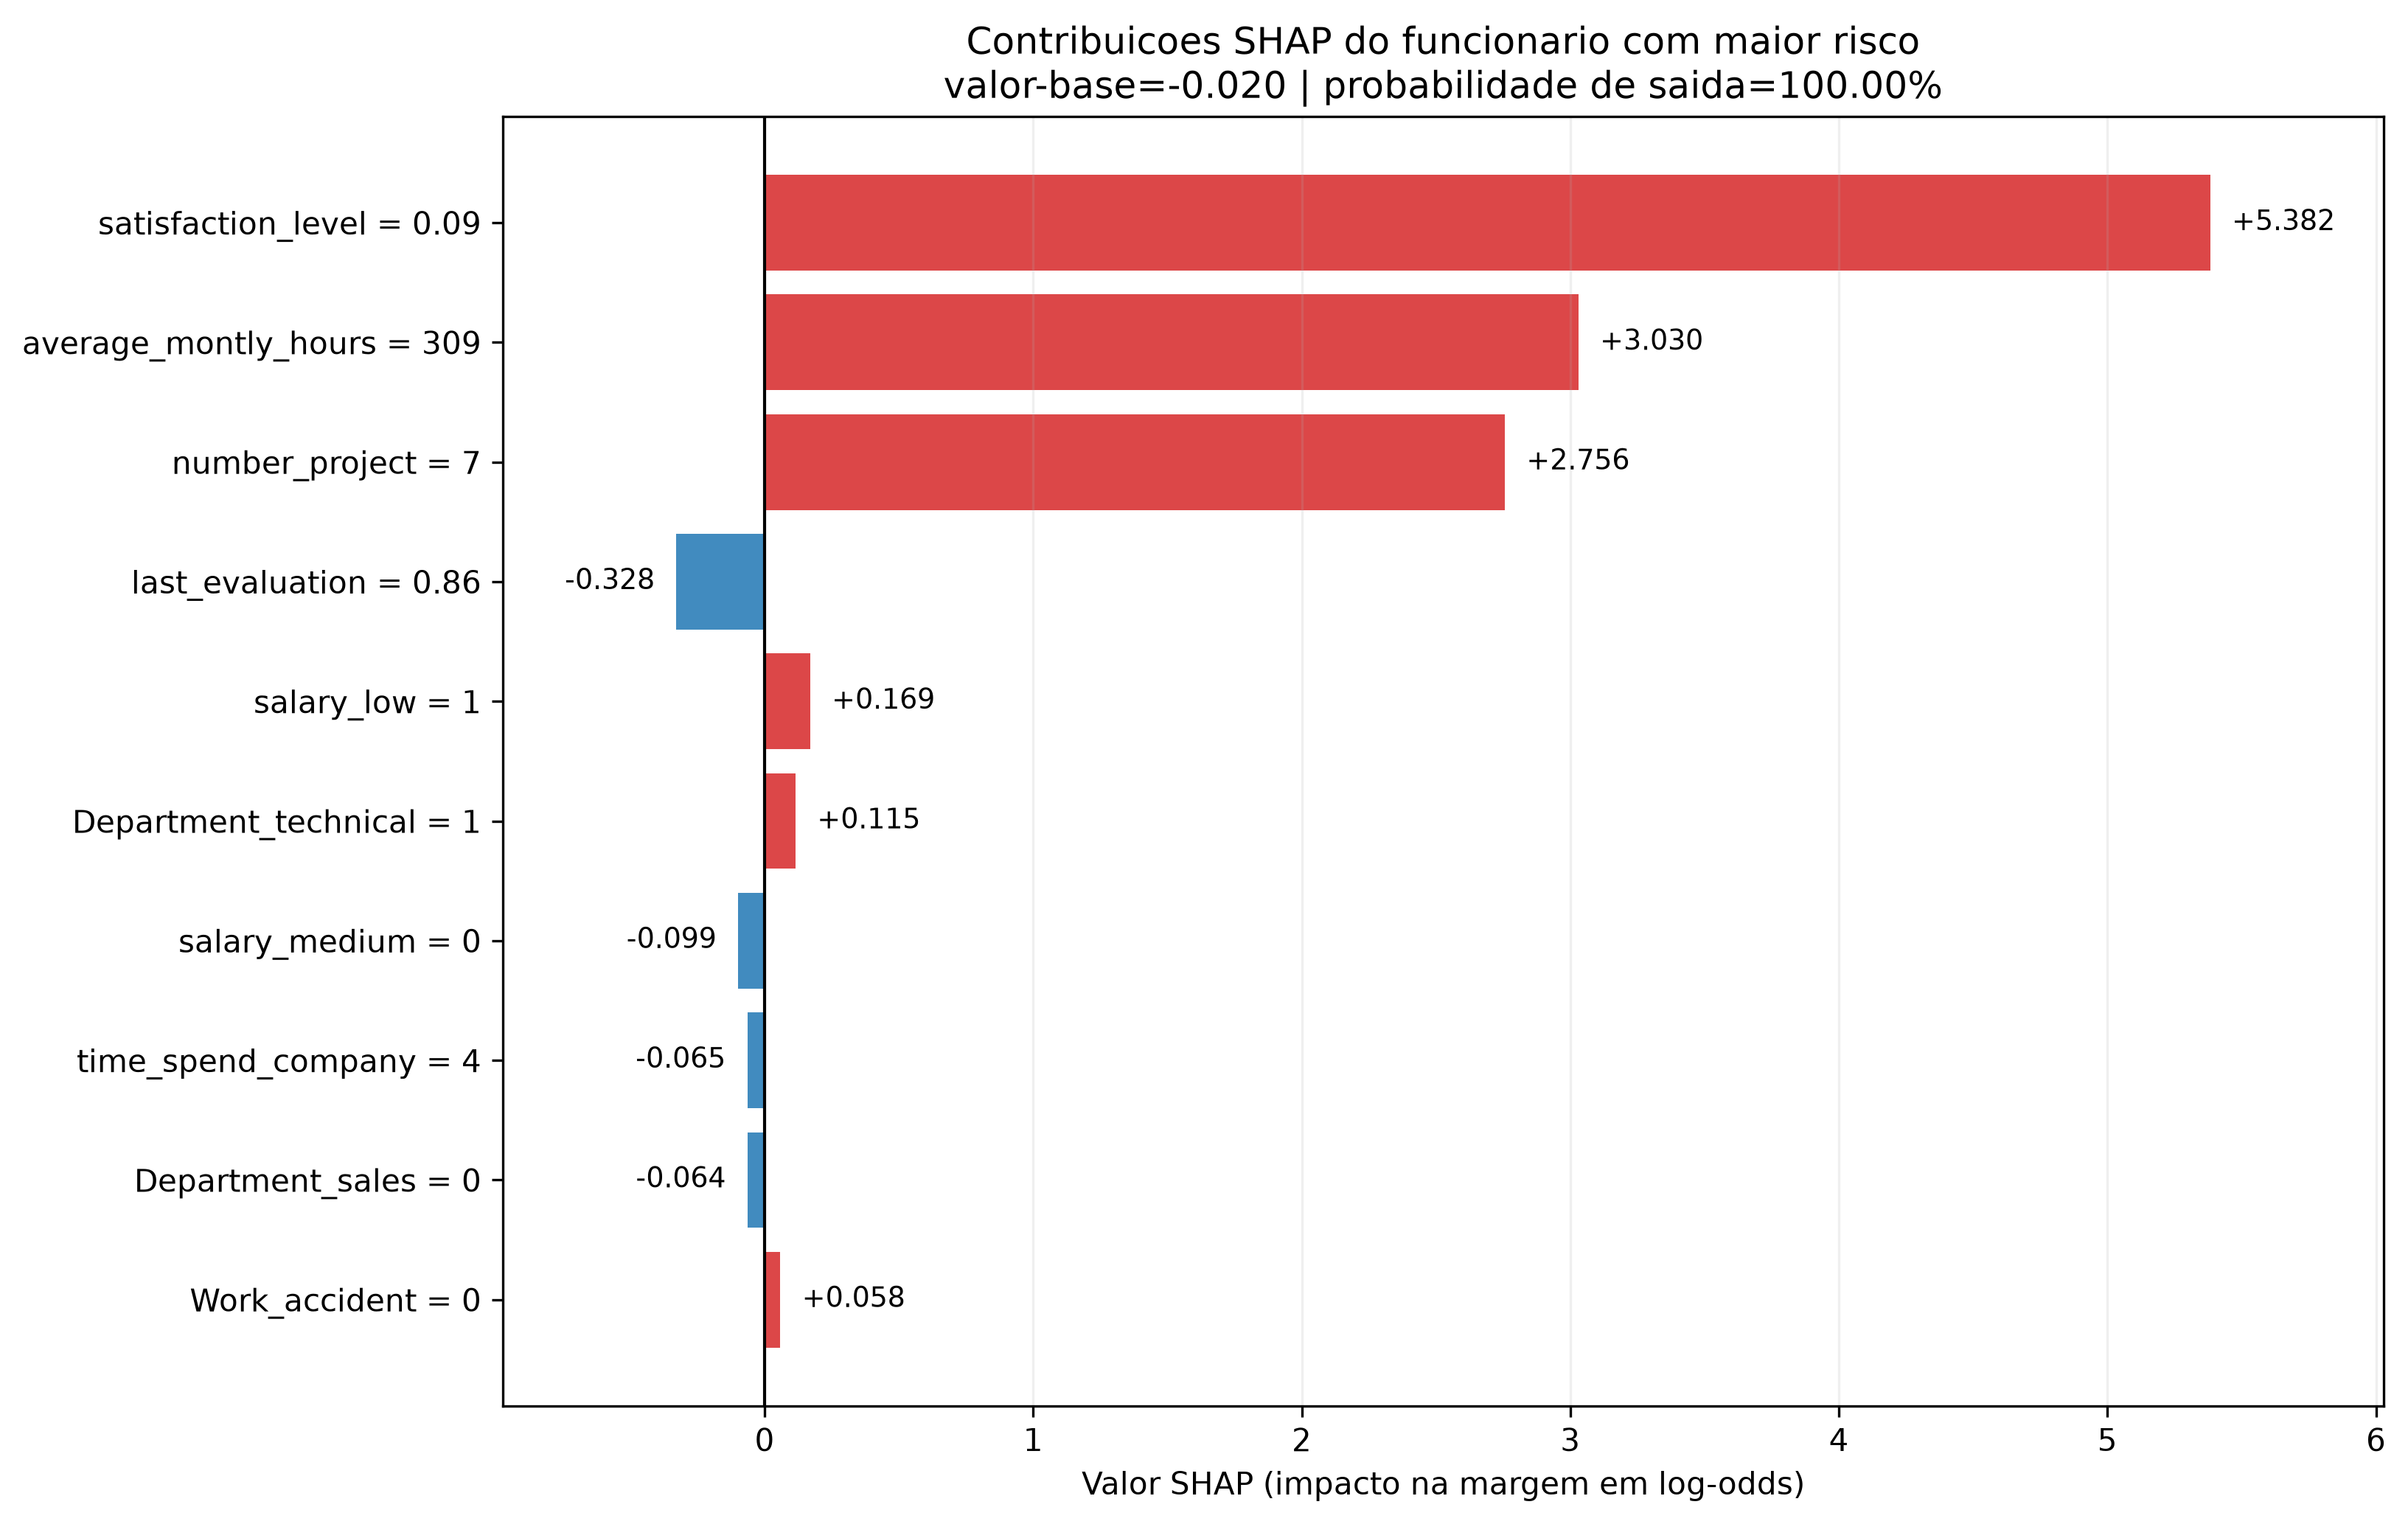
\includegraphics[width=\textwidth]{resultados/shap_maior_risco_xgboost_kfold.png}
\caption{Contribuições SHAP locais de um registro de maior risco.}
\label{fig:shaplocal}
\end{figure}

Os padrões são coerentes com a literatura ao apontar satisfação, carga de trabalho e tempo de empresa como variáveis úteis, mas não comprovam que alterar isoladamente uma delas causará retenção. As contribuições descrevem como o modelo utilizou os dados. Além disso, variáveis correlacionadas podem dividir ou redistribuir importância.

\subsection{Uso dos resultados pelo RH}

O gráfico global é adequado para identificar padrões gerais e formular perguntas organizacionais. O relatório individual permite examinar casos encaminhados como INVESTIGAR. Para evitar a comparação de centenas de parágrafos, foi gerado um relatório intermediário por departamento e faixa salarial. Ele apresenta o tamanho do grupo, a quantidade e o percentual de pessoas sinalizadas pelo limiar de 50\%, o escore médio de saída e fatores SHAP de destaque. Os fatores que aparecem entre os três maiores impactos positivos em todos os grupos com casos sinalizados são apresentados uma única vez por dimensão. Para cada grupo, a tabela destaca até dois fatores com impacto positivo médio maior do que nos demais grupos. As contribuições das colunas categóricas codificadas são somadas antes da comparação por variável original.

No teste final, 694 das 3.000 pessoas foram sinalizadas. Entre os departamentos, o percentual variou de 13,85\% em \texttt{management} a 32,95\% em \texttt{accounting}. Nas faixas salariais, variou de 2,95\% em \texttt{high} a 29,26\% em \texttt{low}. Esses percentuais descrevem classificações do modelo na amostra de teste, não taxas observadas de desligamento nem efeitos causais. O escore médio também não foi calibrado como probabilidade observada. A Figura~\ref{fig:comparativogrupos} apresenta a comparação.

\begin{figure}[ht]
\centering
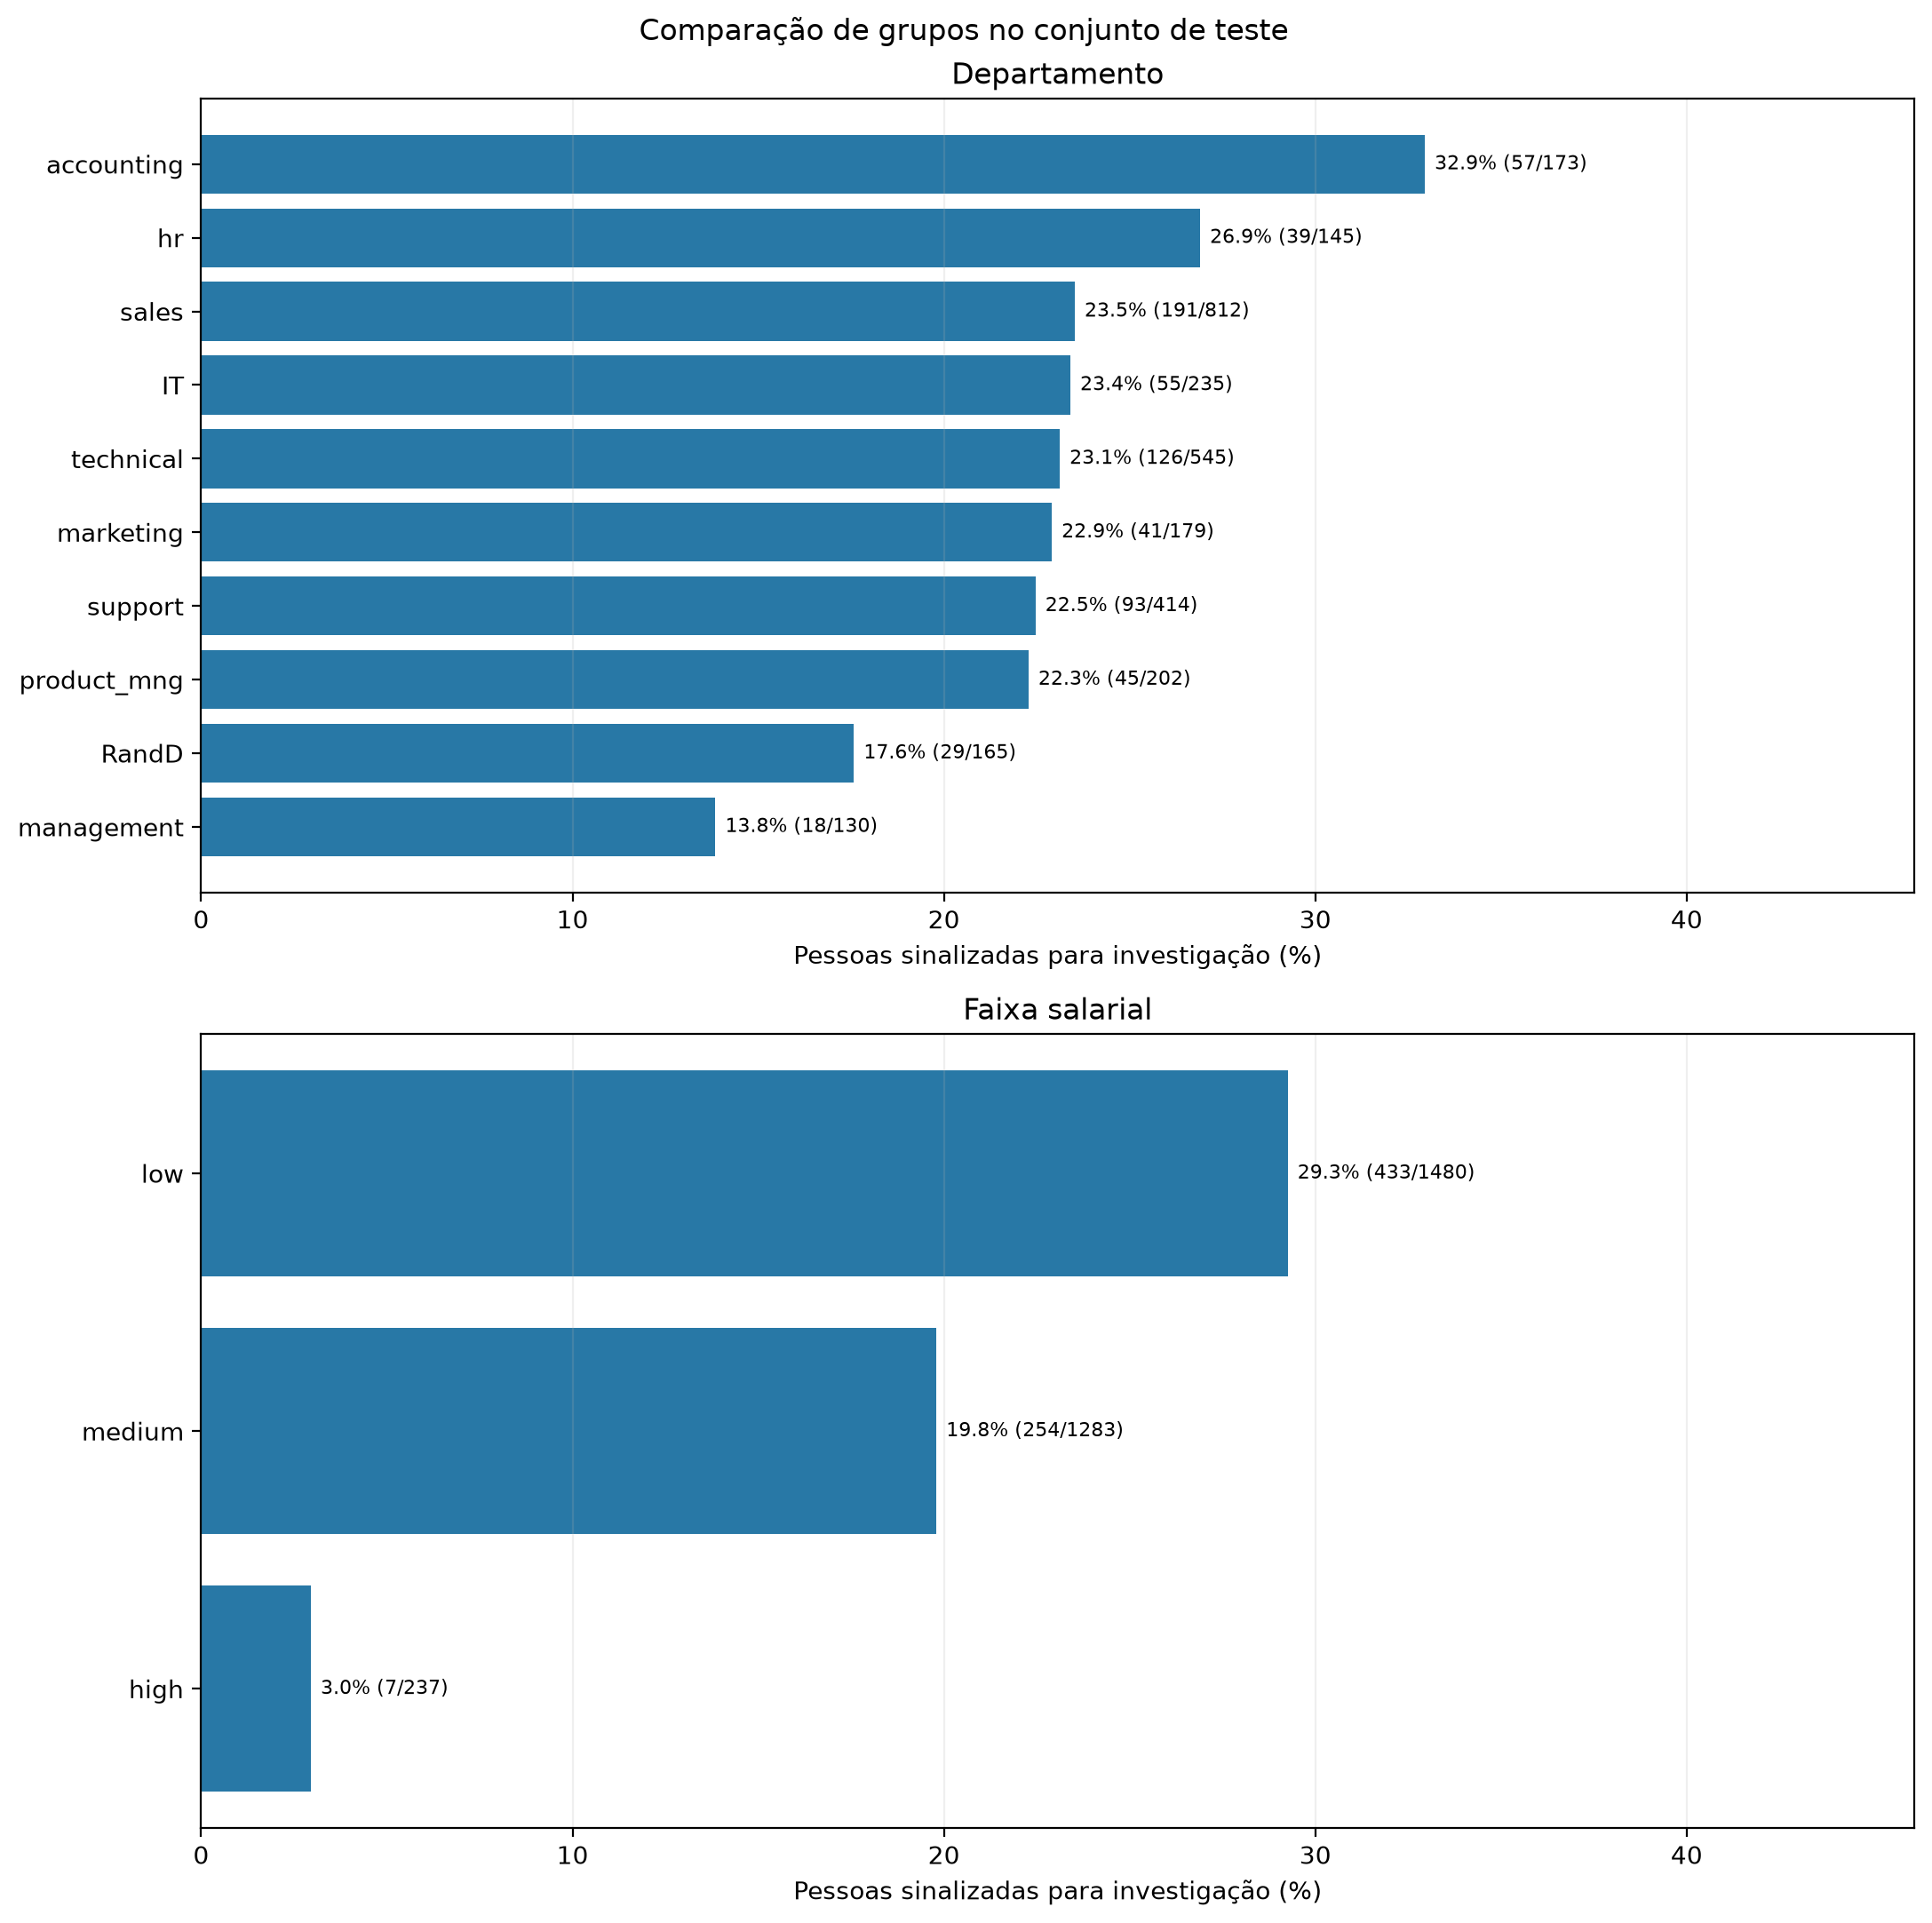
\includegraphics[width=\textwidth]{resultados/comparativo_grupos_rh.png}
\caption{Percentual de pessoas sinalizadas para investigação no conjunto de teste, por departamento e faixa salarial. Os rótulos apresentam casos sinalizados e tamanho de cada grupo.}
\label{fig:comparativogrupos}
\end{figure}

Para aprofundar a análise coletiva, também foi gerado um gráfico SHAP para cada departamento. Os gráficos utilizam todos os registros do respectivo setor no conjunto de teste, não somente as pessoas sinalizadas. Para cada variável original, a implementação soma primeiro as contribuições das categorias codificadas e calcula separadamente as médias dos impactos positivos e negativos. O eixo horizontal mantém a mesma escala em todos os departamentos, permitindo comparar magnitudes. A variável \texttt{Department} é omitida dessas figuras porque define os próprios grupos. A Figura~\ref{fig:shapdepartamento} exemplifica a visualização.

\begin{figure}[ht]
\centering
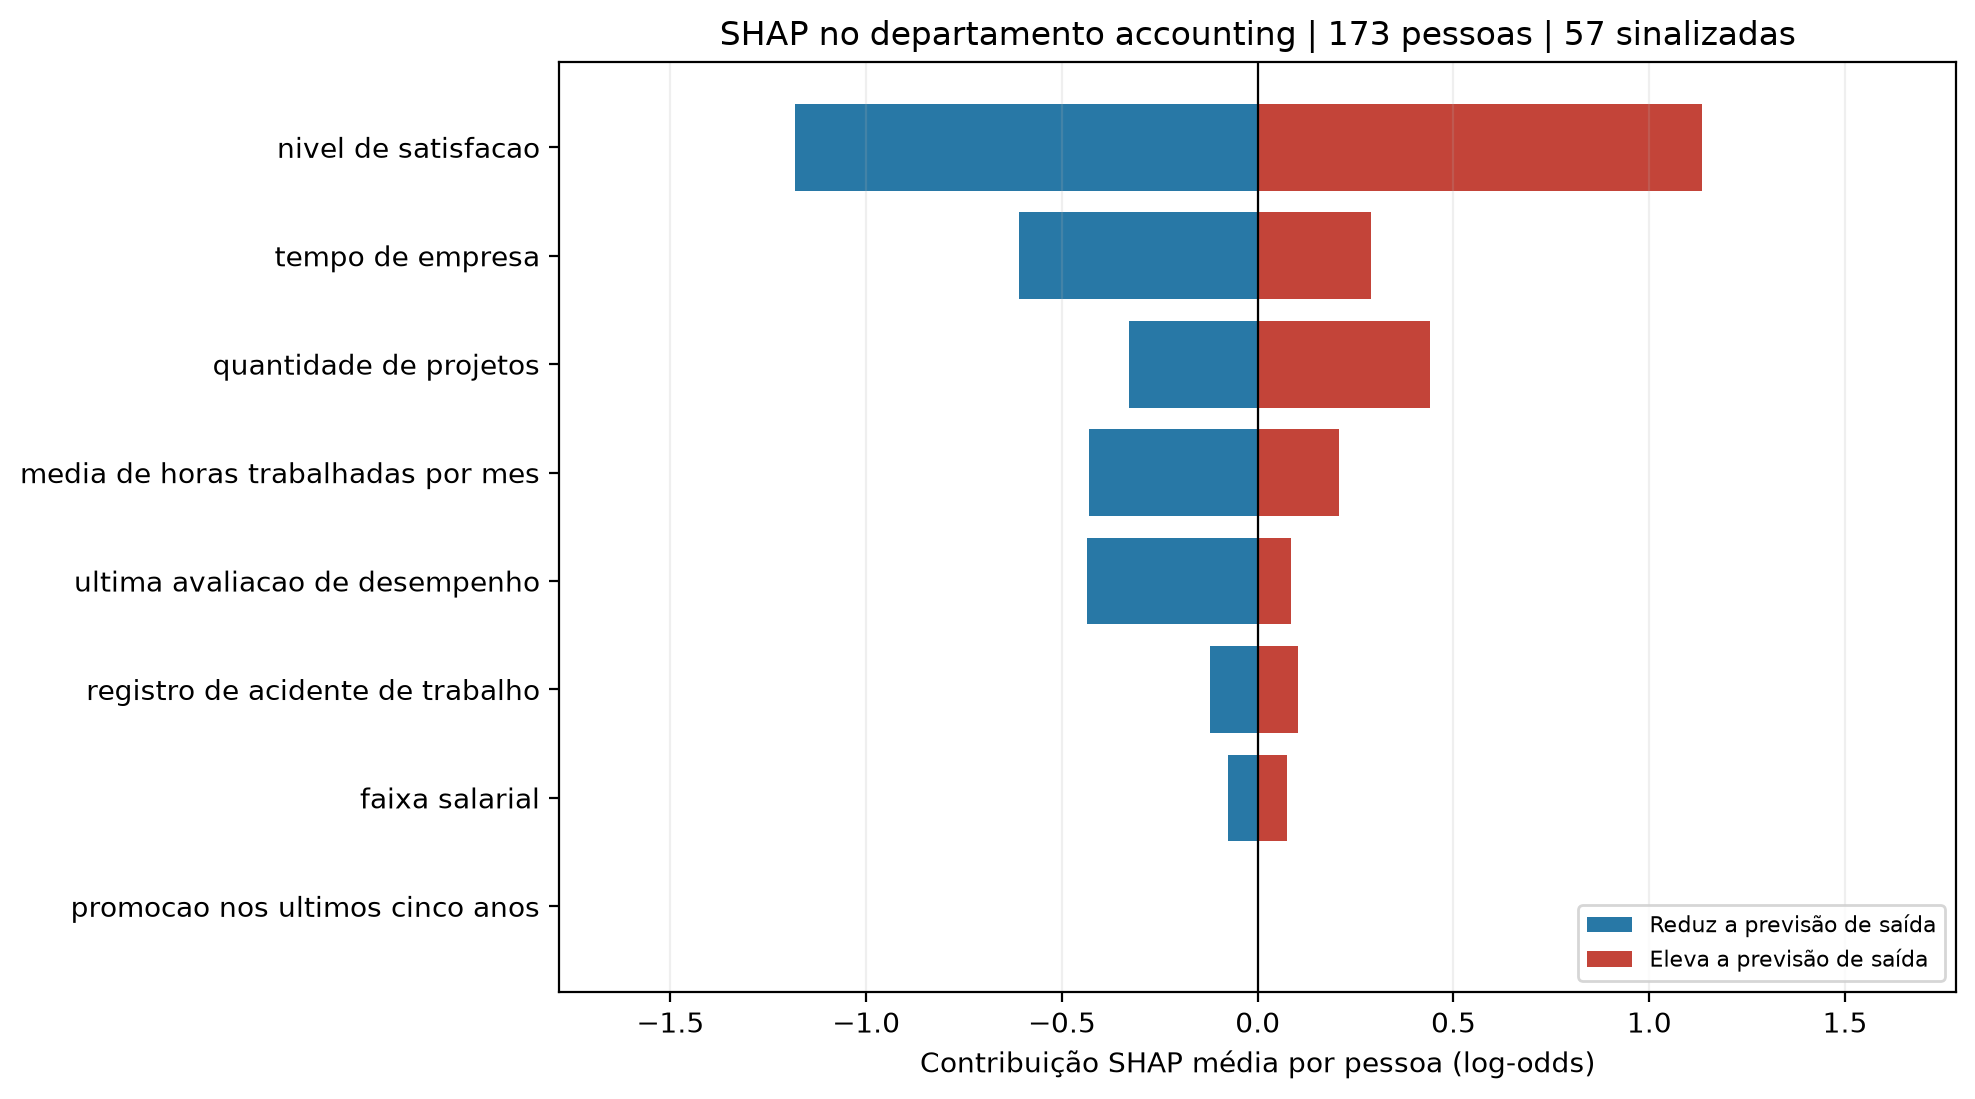
\includegraphics[width=\textwidth]{resultados/shap_departamentos/shap_departamento_accounting.png}
\caption{Contribuições SHAP médias, positivas e negativas, no departamento \texttt{accounting}. Valores em \textit{log-odds}; as duas direções podem ocorrer para uma mesma variável em pessoas diferentes.}
\label{fig:shapdepartamento}
\end{figure}

Um relatório complementar apresenta os fatores que figuram entre os maiores impactos em todos os departamentos uma única vez. O resumo de cada setor destaca até duas características cujo impacto SHAP absoluto médio supera o dos demais setores. O número de pessoas sinalizadas é apresentado separadamente, pois o gráfico SHAP do departamento descreve o grupo inteiro. Essas diferenças são descritivas e não demonstram que o departamento causou as previsões ou os desligamentos.

A LLM permanece opcional. Além das orientações individuais, ela pode selecionar, para cada departamento, uma frase de investigação a partir de uma lista previamente permitida. O programa valida se a resposta corresponde literalmente a um item dessa lista. Totais, percentuais e contribuições numéricas são inseridos pelo programa; a LLM não recebe linhas individuais nesse resumo coletivo. Se ela estiver indisponível ou produzir uma resposta fora do formato esperado, o texto por regras permanece disponível. Essa decisão reduz, mas não elimina, risco de orientação inadequada. Antes de uso real, profissionais de RH devem avaliar clareza, utilidade, consistência e possibilidade de interpretações discriminatórias.

\subsection{Ameaças à validade}

A validade dos resultados é limitada por características da base. Não há documentação suficiente sobre empresa, país, período, política de desligamento ou instrumento que originou satisfação e avaliação. A ausência de \textit{timestamp} impede simular uma previsão verdadeiramente prospectiva, em que o treinamento ocorre no passado e o teste no futuro. A ausência de ID impede acompanhar funcionários e validar se duplicatas são repetições do mesmo indivíduo.

O desempenho elevado pode refletir padrões fortes e repetições específicas desta base. O agrupamento reduz contaminação direta, mas não substitui uma nova amostra externa. Também não há atributos adequados para auditoria ampla de equidade entre grupos protegidos. Por fim, as ações de RH são hipóteses de investigação, não intervenções causalmente validadas.

\section{Conclusões}
\label{sec:conclusoes}

Este trabalho desenvolveu uma abordagem explicável para predição de \textit{turnover} com separação de teste final, validação cruzada estratificada e agrupada, tratamento do desbalanceamento e explicações SHAP. O modelo principal atingiu 97,10\% de acurácia e 92,45\% de \textit{recall} da classe SAIU no teste final. A semelhança entre validação e teste e a baixa variabilidade entre \textit{folds} não indicam sobreajuste acentuado dentro da base analisada.

A comparação mostrou que o XGBoost com peso de classe obteve o melhor equilíbrio no teste, com 97,57\% de acurácia, 97,07\% de precisão e 94,78\% de F1, enquanto o CatBoost apresentou o maior \textit{recall}. As diferenças ainda precisam de avaliação repetida antes da seleção definitiva. As explicações SHAP mostraram que satisfação, tempo de empresa, projetos, horas e avaliação tiveram papel relevante nas previsões do XGBoost.

O resultado deve ser entendido como prova de conceito. A base pública não possui identificação, dimensão temporal ou documentação suficiente para sustentar implantação. Tampouco os valores SHAP demonstram causalidade. Assim, a ferramenta pode priorizar investigações humanas, mas não deve decidir automaticamente sobre pessoas.

Como trabalhos futuros, pretende-se: aplicar SHAP ao XGBoost ponderado; avaliar limiares de classificação conforme custos definidos pelo RH; executar validação cruzada repetida e testes estatísticos; avaliar o relatório comparativo e a redação da LLM com profissionais de RH; realizar auditoria de equidade; e validar o método em dados reais, temporais e externos. Com essas etapas, será possível verificar se o desempenho e as explicações permanecem úteis fora da base utilizada.

\bibliographystyle{sbc}
\bibliography{referencias_tcc}

\end{document}
